\subsection{Finite-time fraction in an operating action annulus}
\label{sec:measure-numerical}
We examine the phase-space fraction defined in
Section~\ref{sec:measure-definition} on a domain spanning millimetre-scale
oscillations. The Hamiltonian is identified from the two-mode COMSOL
position--velocity data in Section~\ref{sec:validated-integral-learning}.
In its canonical coordinates, set
\begin{equation}
 \begin{aligned}
 I_j&=\tfrac12(X_j^2+Y_j^2),\quad j=1,2,\\
 \phi_j&=\operatorname{atan2}(-Y_j,X_j).
 \end{aligned}
 \label{eq:measure-operating-actions}
\end{equation}
and prescribe, before classifying any orbit,
\begin{equation}
 \mathcal D_{\mathrm{op}}=[0.0032,0.0072]^2\times\mathbb T^2_{2\pi}.
 \label{eq:measure-operating-domain}
\end{equation}
Both harmonic modal radii therefore lie in $[0.08,0.12]$, surrounding the
radius $0.1$ of the previously certified $1.898\,\mathrm{mm}$ torus.
The corresponding harmonic tip envelope
$|\ell_1|\sqrt{2I_1}+|\ell_2|\sqrt{2I_2}$ ranges from
$1.518$ to $2.277\,\mathrm{mm}$.
The canonical polar Jacobian has absolute determinant one, so independent
uniform actions and phases sample normalized four-dimensional Liouville volume:
\begin{equation}
 \mu_L(\mathcal D_{\mathrm{op}})
   =(2\pi)^2(0.004)^2=6.3165468\times10^{-4}.
 \label{eq:measure-operating-volume}
\end{equation}
We draw $N=1024$ independent points with PCG64 seed $20261002$; the domain,
initial points, observables, and decision thresholds are specified before
classification. These points are independent of the training observations and the
certified-torus phase grid.

Following weighted Birkhoff averaging~\citep{das2017quasiperiodicity,duignan2023flows},
we compare consecutive windows using the smooth bump
$b(s)=\exp[-1/(s(1-s))]$ for $0<s<1$, with $b=0$ otherwise.
The normalized weighted mean is
\begin{equation}
 W_T(F;z)=\frac{\int_0^T b(t/T)F(\Phi_h^t z)\,dt}
                      {T\int_0^1 b(s)\,ds},
 \label{eq:measure-weighted-average}
\end{equation}
where $\Phi_h^t$ denotes the flow of the fitted Hamiltonian $h$.
The computations use normalized sampled sums of this weight; integration
and quadrature refinements are reported below.
Eight observables are used:
$X_j/0.1$, $Y_j/0.1$, $I_j/0.005$, $X_1X_2/0.01$, and $Y_1Y_2/0.01$.
We also average the polar angular velocities
\begin{equation}
 \dot\phi_j=
 \frac{X_j\partial_{X_j}h+
       Y_j\partial_{Y_j}h}{X_j^2+Y_j^2}.
 \label{eq:measure-angular-frequency}
\end{equation}
For each $T\in\{512,1024,2048,4096\}$, let $e_F(T)$ be the largest
absolute difference of the eight weighted means on $[0,T]$ and $[T,2T]$,
and let $e_\omega(T)$ be the largest relative difference of the two
weighted frequencies. A candidate passes the principal test when
$e_F,e_\omega\le10^{-8}$ at both $T=2048$ and $4096$.
It must also keep both sampled actions above $3.2\times10^{-4}$, have sampled
relative energy drift below $10^{-8}$, and satisfy the finite-order screen
\begin{equation}
 \min_{\substack{0<|k|_1\le64\\k\in\mathbb Z^2\ {\rm primitive}}}
 \frac{|k\cdot\overline\omega|}{|k|_1\|\overline\omega\|_\infty}
 >10^{-7},
 \label{eq:measure-finite-resonance-screen}
\end{equation}
where $\overline\omega$ uses the two longest consecutive windows.
The total simulated time is $8192/\omega_0=717.508\,\mathrm{s}$.
Full cosine and momentum-dependent quartic terms are retained.

Step refinement resolves integration error in the diagnostics. Fixed-step eighth-order DOP853
at $\Delta\tau=1/16$ produces relative energy drift up to $3.94\times10^{-7}$ and
fails the numerical validity test. At $\Delta\tau=1/32$, all points pass the principal
eight-digit criterion and the energy test, but the consecutive-window
averages fail the ten-digit criterion.
Refining all $1024$ trajectories to $\Delta\tau=1/64$, with the same initial
points and thresholds, resolves the ten-digit criterion.
The largest relative energy drift then falls to $6.11\times10^{-12}$;
$e_F(4096)\le4.49\times10^{-12}$ and
$e_\omega(4096)\le3.63\times10^{-14}$.
Halving the step again for the preselected first $64$ points changes no
six-, eight-, or ten-digit labels, with maximum relative frequency change
$2.40\times10^{-14}$. Halving the averaging output interval on identical
saved trajectories changes the weighted means by at most $3.82\times10^{-14}$.
An independent adaptive solver, phase points from the certified torus's
Fourier approximation, an exactly
resonant oscillator, and regular/chaotic two-wave examples provide additional
checks. In particular, the resonant oscillator passes the averaging test but
is rejected by~\eqref{eq:measure-finite-resonance-screen}.

The refined ensemble gives $1024/1024$ candidates at each of the six-, eight-,
and ten-digit thresholds. For the specified finite-time classifier $C$,
\begin{equation}
 \begin{aligned}
 \widehat p_C&=\frac1{1024}\sum_{i=1}^{1024}\mathbf1_C(z_i)=1,\\
 \mathrm{CI}_{95\%}(p_C)&=[0.996404,1].
 \end{aligned}
 \label{eq:measure-empirical-fraction}
\end{equation}
using the two-sided exact Clopper--Pearson interval.
The smallest normalized finite-order detuning is $2.113\times10^{-4}$;
the largest sampled tip displacement is $2.269\,\mathrm{mm}$.
Figure~\ref{fig:measure-finite-time} shows the fixed-domain sample and the
integration and threshold checks.
This interval quantifies only random initial-condition sampling for $C$.
It does not bound classification error, unresolved high-order resonance,
sticky chaos, or physical model error. Thus~\eqref{eq:measure-empirical-fraction}
is an empirical finite-time candidate fraction in the operating domain.
Its $99.6404\%$ lower confidence endpoint concerns the classifier probability,
whereas Appendix~\ref{app:measure-proof} establishes a rigorous KAM-volume
bound on a separate, narrower analytic domain.

\begin{figure*}[t]
 \centering
 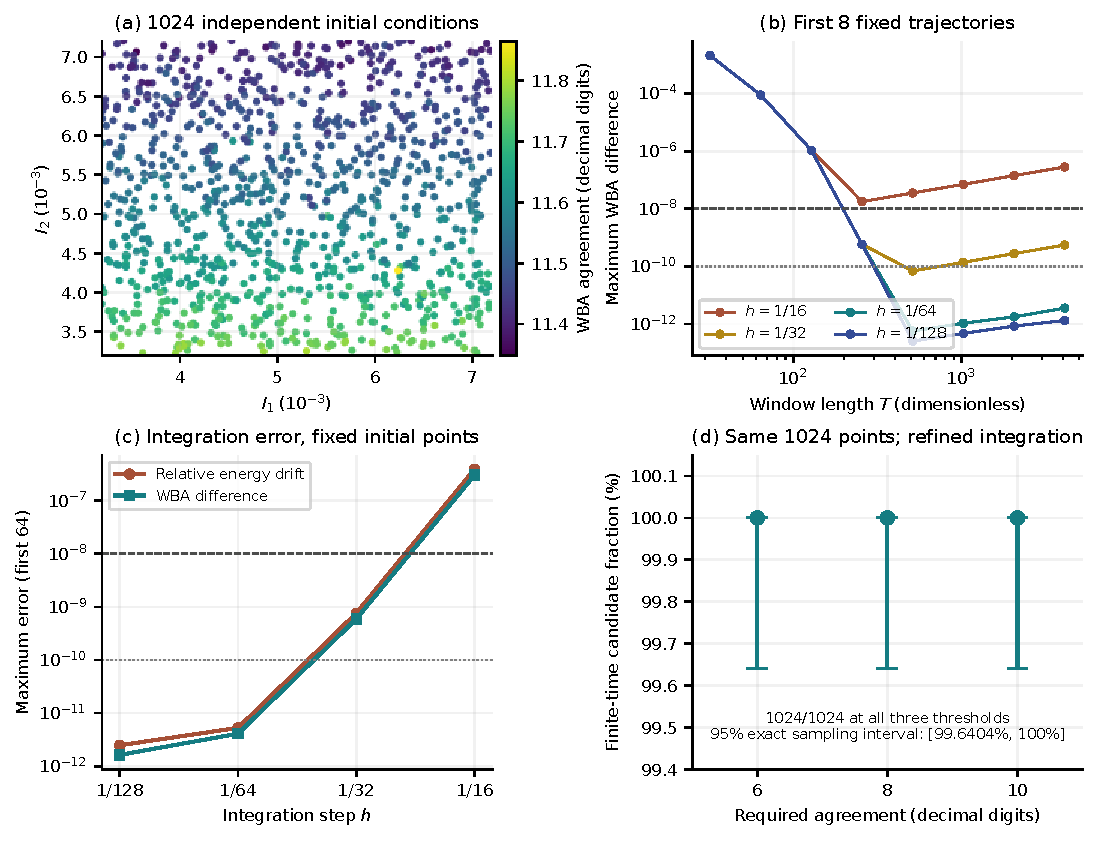
\includegraphics[width=0.95\textwidth]{figures/finite_time_quasiperiodicity.pdf}
 \caption{Finite-time quasiperiodicity diagnostics for the fitted
 Hamiltonian. (a) Uniform action sampling; angles are independently uniform.
 (b) Consecutive-window agreement on the first eight fixed trajectories;
 the long-window floor reflects integration error and roundoff.
 (c) Step refinement on the first $64$ fixed initial points identifies
 the coarse integration error.
 (d) Candidate fractions and exact sampling intervals at three thresholds,
 using the same $1024$ points with refined integration.
 Candidate status describes finite-time agreement of the specified observables.}
 \label{fig:measure-finite-time}
\end{figure*}
